\documentclass[handout]{beamer}
%==============================================================
% Common Beamer Preamble for Course Lectures: Training and Scaling Language Models
%==============================================================

\usepackage[utf8]{inputenc}
\usepackage[T1]{fontenc}
\usepackage{hyperref}
\usepackage{amsmath,amssymb,xcolor,multicol,booktabs,colortbl}
\usepackage{graphicx,listings}
\renewcommand{\figurename}{Figure.}
\renewcommand{\tablename}{Table.}

% ---- TikZ Libraries ----
\usepackage{tikz}
\usetikzlibrary{positioning,arrows.meta,shapes.geometric,calc,fit,backgrounds,decorations.pathreplacing}

% ---- Presentation defaults ----
\setbeamertemplate{navigation symbols}{}
\setbeamersize{text margin left=0.55cm,text margin right=0.55cm}
\setbeamerfont{title}{size=\LARGE,series=\bfseries}
\setbeamerfont{subtitle}{size=\large}

% ---- FontAwesome fallback ----
\IfFileExists{fontawesome5.sty}{%
  \usepackage{fontawesome5}%
}{%
  \providecommand{\faMicrochip}{}%
  \providecommand{\faComments}{}%
  \providecommand{\faTools}{}%
  \providecommand{\faCheckCircle}{}%
  \providecommand{\faExclamationTriangle}{}%
  \providecommand{\faImage}{}%
  \providecommand{\faRobot}{}%
  \providecommand{\faTerminal}{}%
  \providecommand{\faBook}{}%
  \providecommand{\faRedo}{}%
  \providecommand{\faLayerGroup}{}%
  \providecommand{\faCogs}{}%
  \providecommand{\faDatabase}{}%
  \providecommand{\faHdd}{}%
  \providecommand{\faNetworkWired}{}%
}

% ---- Theme Style and Semantic Colors ----
%==============================================================
% Centralized Semantic Color Definitions for LLMs Presentation
%==============================================================

% ---- Base Template / Theme Colors (Aligned with Palette B) ----
\definecolor{themenavy}{RGB}{22,70,102}       % Palette B primary cerulean: #164666
\definecolor{themeblue}{RGB}{22,70,102}       % Primary alias
\definecolor{primarylight}{RGB}{34,92,132}    % Primary light: #225c84
\definecolor{themeteal}{RGB}{0,159,176}       % Accent cyan-teal: #009fb0
\colorlet{main_color}{themenavy}
\colorlet{accent}{themeteal}

\definecolor{accentdark}{RGB}{0,108,120}      % Deep cyan-teal for contrast text
\definecolor{accentlight}{RGB}{56,178,214}    % Slate accent cyan: #38b2d6
\definecolor{leafred}{RGB}{197,93,61}         % Terracotta red for branches/leaves

% ---- Website Panel & Border Neutrals ----
\definecolor{panelbg}{RGB}{237,245,249}       % Course-panel: #edf5f9
\definecolor{panelborder}{RGB}{204,226,238}   % Course-border: #cce2ee

% ---- Code listing style (syntax highlights) ----
\definecolor{deepblue}{RGB}{22,70,102}
\definecolor{deepred}{rgb}{0.6,0,0}
\definecolor{deepgreen}{RGB}{0,135,150}
\definecolor{halfgray}{gray}{0.55}

% ---- Semantic Theme Navy / Cerulean Shades ----
\colorlet{themebluebg}{panelbg}               % Panel #edf5f9
\colorlet{themebluecard}{main_color!8}        % Mild card background fills
\colorlet{themeblueborder}{panelborder}       % Border #cce2ee
\colorlet{themebluemid}{themeteal!60}         % Accent mid-contrast
\colorlet{themebluedraw}{main_color!80}       % Strong outline draws/strokes

% ---- Semantic Secondary Accent Teal Shades ----
\colorlet{accentdarkbg}{themeteal!10}        % Light secondary background fills
\colorlet{accentdarkdraw}{themeteal}         % Secondary outlines/strokes/text/axes

% ---- Functional Colors: Success Green ----
\definecolor{successgreen}{RGB}{55,145,55}
\colorlet{successbg}{successgreen!8}
\colorlet{successdraw}{successgreen!75}

% ---- Functional Colors: Alert Red ----
\definecolor{alertred}{RGB}{197,55,55}
\colorlet{alertbg}{alertred!8}
\colorlet{alertdraw}{alertred!75}

% ---- Functional Colors: Warning Orange ----
\definecolor{warningorange}{RGB}{220,110,30}
\colorlet{warningbg}{warningorange!10}
\colorlet{warningdraw}{warningorange!80}

% ---- Terracotta Red Shades ----
\colorlet{leafredbg}{leafred!12}
\colorlet{leafreddraw}{leafred!80}

% ---- Accent Violet (SWE-bench / observe phases) ----
\definecolor{accentviolet}{RGB}{120,70,180}
\colorlet{accentvioletbg}{accentviolet!10}
\colorlet{accentvioletdraw}{accentviolet!80}

% ---- Post-Training Axis Blue ----
\definecolor{posttrainingblue}{RGB}{40,90,165}
\colorlet{posttrainingbg}{posttrainingblue!8}
\colorlet{posttrainingdraw}{posttrainingblue!75}

% ---- Harness Component Action Green ----
\definecolor{actiongreen}{RGB}{55,145,55}
\colorlet{actiongreenbg}{actiongreen!10}
\colorlet{actiongreendraw}{actiongreen!65}

% ---- Harness Component Persist Olive ----
\definecolor{persistolive}{RGB}{120,135,40}
\colorlet{persistolivebg}{persistolive!12}
\colorlet{persistolivedraw}{persistolive!70}

% ---- Harness Component Observe Violet ----
\colorlet{observevioletbg}{accentvioletbg}
\colorlet{observevioletdraw}{accentvioletdraw}

% ---- Neutrals (Grays/Blacks) ----
\colorlet{neutralbg}{black!4}             % Very light background fills
\colorlet{neutrallight}{black!30}         % Border frames/ticks/dividers
\colorlet{neutraldark}{black!75}          % Main body text/code listing text

% ---- Beamer Block Color Overrides (Premium Terracotta Theme) ----
\setbeamercolor{block title alert}{bg=leafreddraw,fg=white}
\setbeamercolor{block body alert}{bg=leafredbg}
\setbeamercolor{alerted text}{fg=leafreddraw}

\usepackage{../common/style}
\graphicspath{{../common/figs/}{figs/}}

% ---- Code Listing Config ----
\lstset{
  basicstyle=\ttfamily\footnotesize,
  keywordstyle=\bfseries\color{deepblue},
  emphstyle=\ttfamily\color{deepred},
  stringstyle=\color{deepgreen},
  commentstyle=\color{halfgray}\itshape,
  numbers=left, numberstyle=\tiny\color{halfgray},
  backgroundcolor=\color{codebg},
  frame=l, framerule=1.5pt, rulecolor=\color{themeteal},
  xleftmargin=10pt, framexleftmargin=4pt, numbersep=6pt,
  showstringspaces=false, breaklines=true,
  aboveskip=4pt, belowskip=4pt
}

% ---- Image Placeholder Utility ----
\newcommand{\slideimage}[2][3.8cm]{%
  \begin{center}
    \begin{tikzpicture}
      \node[draw=main_color, dashed, very thick, rounded corners,
        fill=themebluebg, minimum width=0.88\linewidth, minimum height=#1,
      text width=0.80\linewidth, align=center, font=\itshape, text=accentdark]
      {\textbf{[ FIGURE / DIAGRAM ]}\\[6pt] #2};
    \end{tikzpicture}
  \end{center}
}

% ---- Concept Highlight Card Utility ----
\newcommand{\conceptcard}[3]{%
  \begin{coursebox}{#1}{#2}#3\end{coursebox}%
}

% ---- Reusable teaching-slide components ----
\newcommand{\learninggoals}[4]{%
  \begin{frame}{What should be clear by the end?}
    \begin{enumerate}
        \setlength{\itemsep}{7pt}
      \item #1
      \item #2
      \item #3
      \item #4
    \end{enumerate}
  \end{frame}
}

\newcommand{\checkpoint}[2]{%
  \begin{frame}{Checkpoint: #1}
    \begin{block}{Think, then compare}
      #2
    \end{block}
  \end{frame}
}

\newcommand{\takeaways}[4]{%
  \begin{frame}{The durable ideas}
    \begin{enumerate}
        \setlength{\itemsep}{8pt}
      \item #1
      \item #2
      \item #3
      \item #4
    \end{enumerate}
  \end{frame}
}

\newcommand{\smallsource}[1]{%
  \vfill\hfill{\tiny\color{neutraldark}Source: #1}
}

% ---- Logo on content frames ----
\newif\ifplacelogo
\placelogotrue
\logo{\ifplacelogo
  \raisebox{-0.3ex}{
\includegraphics[height=0.4cm]{IMT_Atlantique_logo.png}}%
\fi}

\makeatletter
\define@key{beamerframe}{nologo}[true]{%
  \placelogofalse
}
\makeatother

% Fix Beamer bold font warning: substitute undefined T1/cmss/b/n with T1/cmss/bx/n
\DeclareFontShape{T1}{cmss}{b}{n}{<->ssub * cmss/bx/n}{}

% Default Author & Institute metadata
\author[Jonathan Lys]{Jonathan Lys}
\institute[IMT Atlantique]{IMT Atlantique}

% ---- Front Page / Title Slide Macro ----
% Displays Title + IMT Atlantique logo and Brain logo
\newcommand{\makelecturetitle}[1][Training and Scaling Language Models: From First Principles to Efficient Serving]{%
  \placelogofalse
  {
    \setbeamertemplate{footline}{}
    \settitletagline{#1}
    \settitlelogos{%
      \raisebox{-0.5\height}{
\includegraphics[height=1.15cm]{IMT_Atlantique_logo.png}}%
      \hspace{1.2em}%
      \raisebox{-0.5\height}{\includegraphics[height=1.15cm]{brain.pdf}}}
    \begin{frame}[plain]
      \titlepage
    \end{frame}
  }
  \placelogotrue
}

% Section TOC Frame
\AtBeginSection[]{\coursesectiondivider}


\title[TLM -- Session 01]{Session 1: Transformer from First Principles\\[4pt]
\normalsize\itshape Building a Mental Model of a Decoder-Only LM}
\date{\today}

\begin{document}
\makelecturetitle

\begin{frame}{Lecture map}
  \tableofcontents
  \vfill
  \begin{block}{Guiding question}
    What must happen between a token ID and a distribution over the next token?
  \end{block}
\end{frame}

\learninggoals
  {Track the shape and meaning of every tensor in causal self-attention.}
  {Explain why scaling and masking happen before the softmax.}
  {Trace information through a pre-norm decoder block.}
  {Name the tests that make a minimal implementation trustworthy.}

\section{Attention from first principles}

\begin{frame}{Tokens become points in a shared space}
  \begin{columns}[c]
    \begin{column}{0.55\linewidth}
      \begin{itemize}
        \setlength{\itemsep}{7pt}
        \item Input IDs have shape $B\times T$.
        \item A lookup table $W_E\in\mathbb{R}^{V\times d}$ produces content vectors.
        \item Position information makes order visible to the model.
      \end{itemize}
      \[
        X_0 = W_E[\text{ids}] + P_{0:T}
        \quad\in\mathbb{R}^{B\times T\times d}
      \]
    \end{column}
    \begin{column}{0.41\linewidth}
      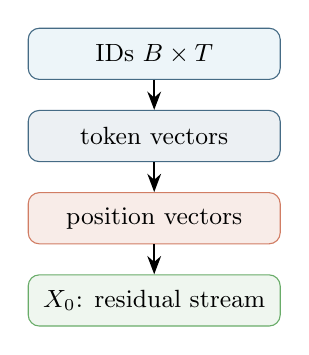
\begin{tikzpicture}[node distance=0.38cm, every node/.style={font=\small}]
        \node[draw=themebluedraw,fill=themebluebg,rounded corners,minimum width=3.2cm,minimum height=.65cm] (ids) {IDs $B\times T$};
        \node[draw=themebluedraw,fill=themebluecard,rounded corners,below=of ids,minimum width=3.2cm,minimum height=.65cm] (tok) {token vectors};
        \node[draw=leafreddraw,fill=leafredbg,rounded corners,below=of tok,minimum width=3.2cm,minimum height=.65cm] (pos) {position vectors};
        \node[draw=successdraw,fill=successbg,rounded corners,below=of pos,minimum width=3.2cm,minimum height=.65cm] (x) {$X_0$: residual stream};
        \draw[-{Stealth},thick] (ids)--(tok);
        \draw[-{Stealth},thick] (tok)--(pos);
        \draw[-{Stealth},thick] (pos)--(x);
      \end{tikzpicture}
    \end{column}
  \end{columns}
\end{frame}

\begin{frame}{Attention is learned retrieval}
  \begin{columns}[t]
    \begin{column}{0.31\linewidth}
      \begin{block}{Query}
        What does this position need?
        \[Q=XW_Q\]
      \end{block}
    \end{column}
    \begin{column}{0.31\linewidth}
      \begin{block}{Key}
        What does each position offer?
        \[K=XW_K\]
      \end{block}
    \end{column}
    \begin{column}{0.31\linewidth}
      \begin{block}{Value}
        What content should move?
        \[V=XW_V\]
      \end{block}
    \end{column}
  \end{columns}
  \vspace{5pt}
  \[
    \operatorname{Attn}(Q,K,V)
    = \operatorname{softmax}\!\left(\frac{QK^\top}{\sqrt{d_h}}+M\right)V
  \]
  \begin{alertblock}{The distinction that matters}
    Queries and keys choose the mixture. Values supply the mixed information.
  \end{alertblock}
  \smallsource{Vaswani et al. and The Annotated Transformer}
\end{frame}

\begin{frame}{Why divide by $\sqrt{d_h}$?}
  Assume independent query and key components with unit variance.
  \[
    q^\top k = \sum_{i=1}^{d_h} q_i k_i
    \qquad
    \operatorname{Var}(q^\top k)\approx d_h
  \]
  \begin{columns}[c]
    \begin{column}{0.47\linewidth}
      \begin{alertblock}{Without scaling}
        Wider heads create larger logits. Softmax saturates and gradients become poorly conditioned.
      \end{alertblock}
    \end{column}
    \begin{column}{0.47\linewidth}
      \begin{block}{With scaling}
        Dividing by $\sqrt{d_h}$ keeps logit variance roughly constant across head widths.
      \end{block}
    \end{column}
  \end{columns}
  \vfill
  \centering\textbf{This is a variance-control argument, not a cosmetic constant.}
\end{frame}

\begin{frame}{Causality is a constraint on logits}
  \begin{columns}[c]
    \begin{column}{0.48\linewidth}
      \centering
      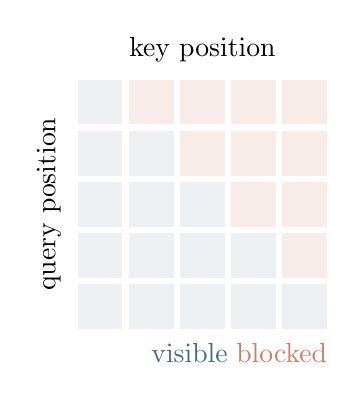
\begin{tikzpicture}[scale=.65]
        \foreach \i in {0,...,4}{
          \foreach \j in {0,...,4}{
            \pgfmathparse{int(\j<=\i)}
            \ifnum\pgfmathresult=1
              \fill[themebluecard] (\j,-\i) rectangle +(0.9,-0.9);
            \else
              \fill[leafredbg] (\j,-\i) rectangle +(0.9,-0.9);
            \fi
            \draw[white] (\j,-\i) rectangle +(0.9,-0.9);
          }
        }
        \node[above] at (2.45,.15) {key position};
        \node[rotate=90] at (-.55,-2.45) {query position};
        \node[themebluedraw] at (2.2,-5.35) {visible};
        \node[leafreddraw] at (4.0,-5.35) {blocked};
      \end{tikzpicture}
    \end{column}
    \begin{column}{0.48\linewidth}
      \begin{itemize}
        \setlength{\itemsep}{8pt}
        \item Position $t$ may use keys $0\ldots t$.
        \item Future logits receive $-\infty$ before softmax.
        \item Masking probabilities after softmax breaks normalization.
      \end{itemize}
      \begin{block}{Causality test}
        Change one future token. Earlier output logits must remain identical.
      \end{block}
    \end{column}
  \end{columns}
\end{frame}

\checkpoint{one query row}
  {For sequence length four, write the four logits seen by the query at position two. Which entries survive the mask, and across which dimension must softmax normalize?}

\section{The decoder block}

\begin{frame}{Multiple heads create multiple retrieval spaces}
  \begin{columns}[c]
    \begin{column}{0.54\linewidth}
      \begin{align*}
        d_h &= d / H \\
        Q,K,V &: B\times H\times T\times d_h \\
        S=QK^\top &: B\times H\times T\times T \\
        \operatorname{concat}(O_h) &: B\times T\times d
      \end{align*}
      Heads run the same operation with different learned projections. The output projection mixes their results back into the residual stream.
    \end{column}
    \begin{column}{0.42\linewidth}
      \begin{alertblock}{Shape invariant}
        $d$ must be divisible by $H$. A transpose mistake can preserve element count while changing semantics.
      \end{alertblock}
      \begin{block}{Useful habit}
        Annotate batch, head, query, key, and channel axes before every reshape.
      \end{block}
    \end{column}
  \end{columns}
\end{frame}

\begin{frame}{A pre-norm block has two residual updates}
  \begin{columns}[c]
    \begin{column}{0.52\linewidth}
      \[
        X' = X + \operatorname{MHA}(\operatorname{Norm}(X))
      \]
      \[
        X'' = X' + \operatorname{MLP}(\operatorname{Norm}(X'))
      \]
      \begin{itemize}
        \setlength{\itemsep}{7pt}
        \item Attention mixes information across positions.
        \item The MLP transforms each position independently.
        \item Residual paths preserve a direct information route.
      \end{itemize}
    \end{column}
    \begin{column}{0.44\linewidth}
      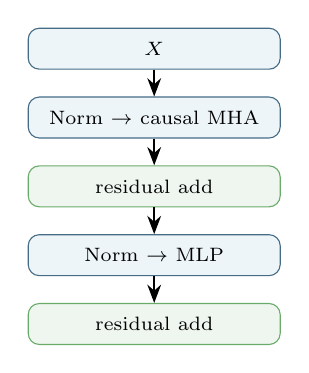
\begin{tikzpicture}[node distance=.34cm,every node/.style={font=\scriptsize},box/.style={draw=themebluedraw,fill=themebluebg,rounded corners,minimum width=3.2cm,minimum height=.52cm}]
        \node[box] (x) {$X$};
        \node[box,below=of x] (n1) {Norm $\rightarrow$ causal MHA};
        \node[box,fill=successbg,draw=successdraw,below=of n1] (a) {residual add};
        \node[box,below=of a] (n2) {Norm $\rightarrow$ MLP};
        \node[box,fill=successbg,draw=successdraw,below=of n2] (b) {residual add};
        \draw[-{Stealth},thick] (x)--(n1);
        \draw[-{Stealth},thick] (n1)--(a);
        \draw[-{Stealth},thick] (a)--(n2);
        \draw[-{Stealth},thick] (n2)--(b);
      \end{tikzpicture}
    \end{column}
  \end{columns}
\end{frame}

\begin{frame}{Pre-norm and post-norm are different models}
  \begin{columns}[t]
    \begin{column}{0.47\linewidth}
      \begin{block}{Pre-norm}
        \[X + F(\operatorname{Norm}(X))\]
        The identity path bypasses normalization. Deep optimization is usually more forgiving.
      \end{block}
    \end{column}
    \begin{column}{0.47\linewidth}
      \begin{alertblock}{Post-norm}
        \[\operatorname{Norm}(X + F(X))\]
        This is the original Transformer form. It has a different gradient path and training behavior.
      \end{alertblock}
    \end{column}
  \end{columns}
  \vfill
  \centering\textbf{Do not describe one convention and implement the other.}
\end{frame}

\begin{frame}{The language-model head turns states into a task}
  \begin{columns}[c]
    \begin{column}{0.55\linewidth}
      \[
        Z = \operatorname{Norm}(X_N)W_{\text{vocab}}^\top
        \quad\in\mathbb{R}^{B\times T\times V}
      \]
      \[
        \mathcal{L}=-\frac{1}{BT}\sum_{b,t}
        \log p(x_{b,t+1}\mid x_{b,0:t})
      \]
      Each position predicts the next token. The target is the input shifted by one position.
    \end{column}
    \begin{column}{0.41\linewidth}
      \begin{block}{One stream, two views}
        \texttt{x = tokens[:, :-1]}\\[5pt]
        \texttt{y = tokens[:, 1:]}
      \end{block}
      \begin{alertblock}{Common bug}
        A wrong shift can produce a finite, decreasing loss while training the wrong task.
      \end{alertblock}
    \end{column}
  \end{columns}
\end{frame}

\section{Evidence before scale}

\begin{frame}{A shape ledger catches semantic bugs}
  \centering\small
  \begin{tabular}{lll}
    \toprule
    Tensor & Shape & Meaning \\
    \midrule
    token IDs & $B\times T$ & discrete input \\
    residual stream & $B\times T\times d$ & one state per position \\
    $Q,K,V$ & $B\times H\times T\times d_h$ & per-head projections \\
    attention scores & $B\times H\times T\times T$ & query-key compatibility \\
    head output & $B\times H\times T\times d_h$ & contextualized values \\
    logits & $B\times T\times V$ & next-token scores \\
    \bottomrule
  \end{tabular}
  \vfill
  \begin{block}{Review question}
    Which axis does softmax consume, and which reshape reconstructs $d$ without mixing tokens?
  \end{block}
\end{frame}

\begin{frame}{Three tests establish a trustworthy baseline}
  \begin{enumerate}
    \setlength{\itemsep}{9pt}
    \item \textbf{Shape test}: every intermediate matches the ledger for several $B,T,H$ values.
    \item \textbf{Causality test}: modifying a future token cannot change earlier logits.
    \item \textbf{Tiny-batch overfit}: a small model drives loss near zero on one repeated batch.
  \end{enumerate}
  \begin{alertblock}{What each failure means}
    Shape failure suggests layout. Causality failure suggests masking. Overfit failure suggests optimization, targets, or the end-to-end data path.
  \end{alertblock}
\end{frame}

\begin{frame}{The same components support three model families}
  \begin{columns}[t]
    \begin{column}{0.31\linewidth}
      \begin{block}{Encoder-only}
        Bidirectional attention produces representations for understanding tasks.
      \end{block}
    \end{column}
    \begin{column}{0.31\linewidth}
      \begin{block}{Encoder--decoder}
        A source encoder connects to a causal decoder through cross-attention.
      \end{block}
    \end{column}
    \begin{column}{0.31\linewidth}
      \begin{block}{Decoder-only}
        One causal token stream defines next-token prediction and generation.
      \end{block}
    \end{column}
  \end{columns}
  \vfill
  Modern LLMs vary attention type, position method, normalization, MLP, and sparsity while retaining this core residual architecture.
\end{frame}

\checkpoint{debugging order}
  {A model runs and loss decreases slowly, but generation copies future tokens from the training sequence. Which test should have caught this, and which tensors would you inspect first?}

\takeaways
  {Attention performs content-addressed mixing through queries, keys, and values.}
  {Scaling stabilizes logits. Causal masking protects the prediction task.}
  {A decoder block alternates cross-token mixing and per-token transformation.}
  {Shapes, causality, and tiny-batch overfitting are the minimum evidence.}

\end{document}
